\chapter{Physical Design}
\label{pd}
The physical design of the unit has been achieved by the usage of a script (Appendix \ref{appendix12}). As for the synthesis, this script is in charge of preparing the environment and start the real script for the physical design.\\ This step is very well known as a computing intensive step, even more then the synthesis since the granularity of details is bigger than the one in the synthesis. Therefore, for boosting-up the performance the script automatically sets the usage of six threads instead of only one.\\\\
Nevertheless the variety in the design space, only a subset of them has been choosen for being placed on a die. In particular the unconstrained desing, the minimum area and a 10\% less of the clock frequency and only the 10\% less of the clock frequency designs. It is worth to mention that the physical design does not use the RTL description but it uses the gate-level netlist of the RTL, produced by the synthesis.\\
\section{Results}
In the following pages, results are presented as images of the design on the same die.

\begin{figure}[!htbp]
  \centering
  \begin{subfigure}[b]{0.4\linewidth}
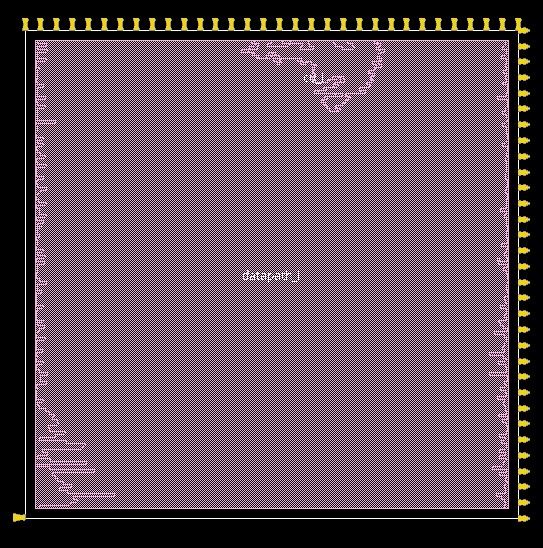
\includegraphics[width=\linewidth,scale=0.5,angle=0]{../project/physical_design/images_nopt/DLX_IR_SIZE32_PC_SIZE32_nopt_ameba_prerouting.jpg}
\caption{Ameba view of unconstrained design}
\label{fig:amebano}
  \end{subfigure}
  \begin{subfigure}[b]{0.4\linewidth}
   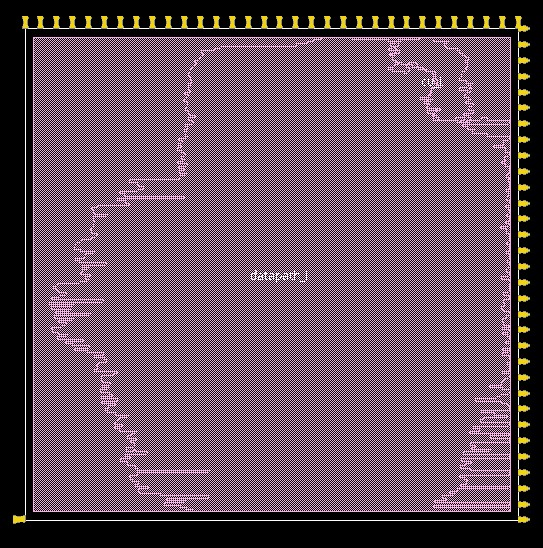
\includegraphics[width=\linewidth,scale=0.5,angle=0]{../project/physical_design/images_10/DLX_IR_SIZE32_PC_SIZE32_10_ameba_prerouting.jpg}
\caption{Ameba view of design with 10\% less on clock frequency}
\label{fig:ameba10}
  \end{subfigure}

  \label{fig:ameba}
\end{figure}


\begin{figure}[!htbp]
\centering
\captionsetup{justification=centering}
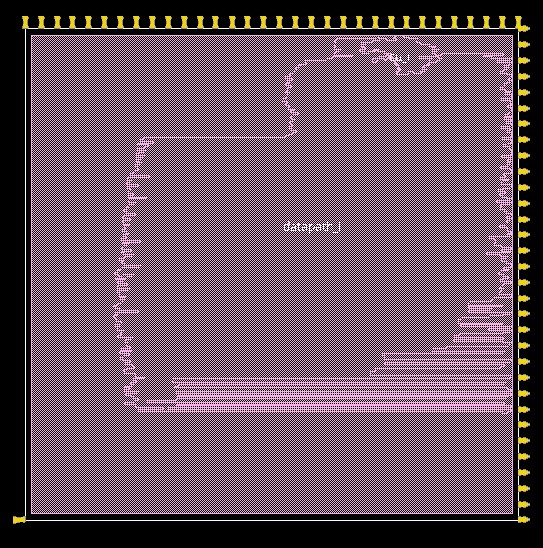
\includegraphics[scale=0.5,angle=0]{../project/physical_design/images_1_minarea/DLX_IR_SIZE32_PC_SIZE32_1_minarea_ameba_prerouting.jpg}
\caption{Ameba view of design with 1\% less on clock frequency and minimum area}
\label{fig:ameba1minarea}
\end{figure}


\begin{figure}[!htbp]
\centering
\captionsetup{justification=centering}
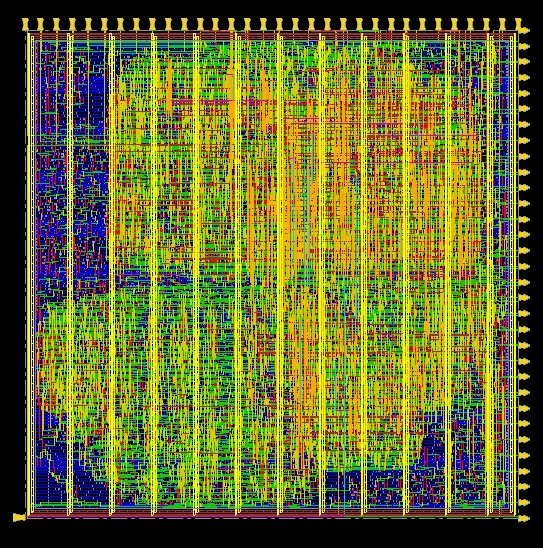
\includegraphics[scale=0.5,angle=0]{../project/physical_design/images_nopt/DLX_IR_SIZE32_PC_SIZE32_nopt_place_prerouting.jpg}
\caption{Placement of unconstrained design}
\label{fig:placno}
\end{figure}




\begin{figure}[!htbp]
\centering
\captionsetup{justification=centering}
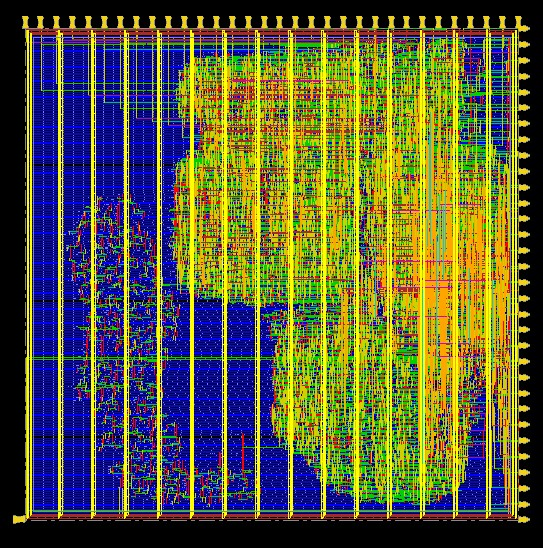
\includegraphics[scale=0.5,angle=0]{../project/physical_design/images_10/DLX_IR_SIZE32_PC_SIZE32_10_place_prerouting.jpg}
\caption{Placement of design with 10\% less on clock frequency}
\label{fig:plac10}
\end{figure}






\begin{figure}[!htbp]
\centering
\captionsetup{justification=centering}
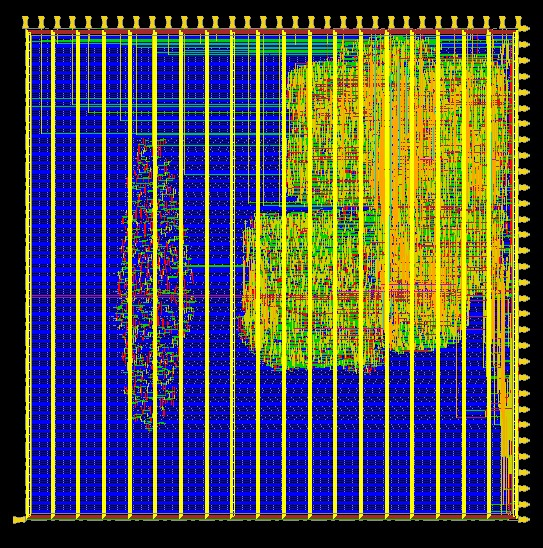
\includegraphics[scale=0.5,angle=0]{../project/physical_design/images_1_minarea/DLX_IR_SIZE32_PC_SIZE32_1_minarea_place_prerouting.jpg}
\caption{Placement of design with 1\% less on clock frequency and minumum area}
\label{fig:plac1minarea}
\end{figure}
